%%%%%%%%%%%%%%%%%%%%%%%%%%%%%%%%%%%%%%%%%
% Beamer Presentation
% LaTeX Template
% Version 1.0 (10/11/12)
%
% This template has been downloaded from:
% http://www.LaTeXTemplates.com
%
% License:
% CC BY-NC-SA 3.0 (http://creativecommons.org/licenses/by-nc-sa/3.0/)
%
%%%%%%%%%%%%%%%%%%%%%%%%%%%%%%%%%%%%%%%%%

%----------------------------------------------------------------------------------------
%	PACKAGES AND THEMES
%----------------------------------------------------------------------------------------

\documentclass[aspectratio=169]{beamer}

\mode<presentation> {

\usetheme{CambridgeUS}

}

\usepackage{color}
\usepackage{graphicx} % Allows including images
\usepackage{url}
\usepackage{hyperref}
\usepackage{algorithm2e}
\DontPrintSemicolon

\DeclareGraphicsExtensions{.png}

\setlength{\parskip}{1em}

%----------------------------------------------------------------------------------------
%	TITLE PAGE
%----------------------------------------------------------------------------------------

\title[Complexity theory]{An introduction to complexity theory} % The short title appears at the bottom of every slide, the full title is only on the title page

\author{Dominic Moylett} % Your name
\institute[University of Bristol] % Your institution as it will appear on the bottom of every slide, may be shorthand to save space
{
University of Bristol \\ % Your institution for the title page
\medskip
\textit{dominic.moylett@bristol.ac.uk} % Your email address
}
\date{\today} % Date, can be changed to a custom date

\begin{document}

\begin{frame}
\titlepage % Print the title page as the first slide
\end{frame}

%----------------------------------------------------------------------------------------
%	PRESENTATION SLIDES
%----------------------------------------------------------------------------------------

%------------------------------------------------
\section{Introduction: What is complexity theory?}
%------------------------------------------------

\begin{frame}
\frametitle{Complexity theory in a nutshell}
\centerline{``How hard can it be?'', {\em Jeremy Clarkson}}
\end{frame}

\begin{frame}
\frametitle{What is complexity theory?}
Complexity theory is the study of how difficult it is to solve a problem with a computer.
\end{frame}

\begin{frame}
\frametitle{What is complexity theory?}
Complexity theory is the study of how {\color{red} difficult} it is to solve a problem with a computer.

How do we measure difficulty?
\end{frame}

\begin{frame}
\frametitle{What is complexity theory?}
Complexity theory is the study of how difficult it is to solve a {\color{red} problem} with a computer.

What do we mean when we talk about a problem?
\end{frame}

\begin{frame}
\frametitle{What is complexity theory?}
Complexity theory is the study of how difficult it is to solve a problem with a {\color{red} computer}.

What do we mean when we talk about a computer?
\end{frame}

\begin{frame}
\frametitle{Structure of part one}
\begin{itemize}
    \item What is a computer?
    \item What is a problem?
    \item How do we measure difficulty?
\end{itemize}
\end{frame}

%------------------------------------------------
\section{Summary of part one}
%------------------------------------------------

\begin{frame}
\frametitle{Summary of part one}
\begin{itemize}
    \item What is a computer? {\em Deterministic Turing Machine, Non-Deterministic Turing Machine}
    \item What is a problem? {\em Deciding if a word is in a language, verifying that a word is in a language}
    \item How do we measure difficulty? {\em Upper bound of time for an input of length $n$}
\end{itemize}
\end{frame}

%------------------------------------------------
\section{End of part one}
%------------------------------------------------

\begin{frame}
\frametitle{End of part one}
\begin{center}
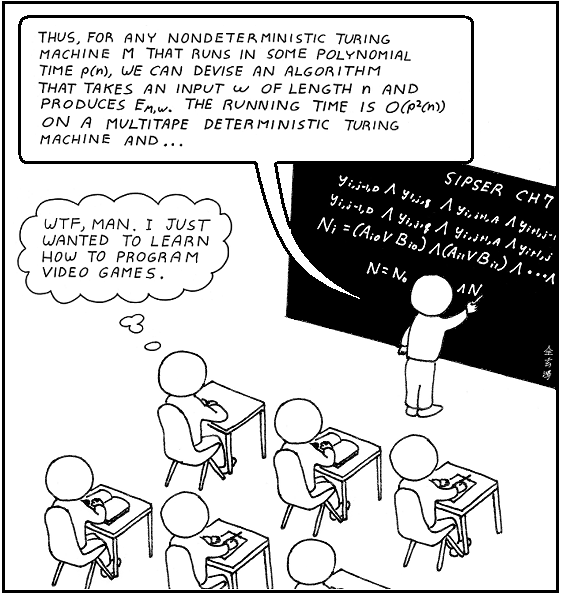
\includegraphics[scale=0.3]{ag_comic}\footnote{\url{http://abstrusegoose.com/206}}
\end{center}
\end{frame}

%------------------------------------------------
\section{Structure of part two}
%------------------------------------------------

\begin{frame}
\frametitle{Structure of part two}
\begin{itemize}
    \item Putting it all together!
    \item ...only to get another (very difficult) problem.
    \item How might we try to solve this new problem?
\end{itemize}
\end{frame}

%------------------------------------------------
\section{The $P$ versus $NP$ problem}
%------------------------------------------------

\begin{frame}
\frametitle{Exercise Left for the Student}
\centerline{Does $P=NP$?}

(NB: You should probably refer to the literature before trying to solve this.)
\end{frame}

\begin{frame}
\frametitle{The $P$ versus $NP$ problem}
Arguably first proposed by G\"{o}del in a letter to von Neumann in 1956.\footnote{\url{https://ecommons.cornell.edu/bitstream/handle/1813/6910/89-994.pdf}}

First stated formally by Cook in 1971.\footnote{\url{http://dl.acm.org/citation.cfm?coll=GUIDE&dl=GUIDE&id=805047}}

Solving the problem will earn you a million dollars, courtesy of the Clay Institute.\footnote{\url{http://www.claymath.org/millennium-problems}}

Aaronson has called it the most important Millenium Problem, as the answer could make the other problems significantly easier or harder to solve.\footnote{\url{http://www.thenakedscientists.com/HTML/interviews/interview/1001376/}}
\end{frame}

\begin{frame}
\frametitle{The easy side: $P \subseteq NP$}

Recall that any $TM$ is by definition non-deterministic.

Likewise, any polynomial-time $TM$ is also non-deterministic.

So $\forall L \in P, L \in NP$. Hence $P \subseteq NP$.
\end{frame}

\begin{frame}
\frametitle{The easy side: $P \subseteq NP$}

Alternative proof (using verification):

Let $TM\, M$ decide $L$ in polynomial time. Define $V$ as follows:

\begin{algorithm}[H]
$V(w, c):$\\
\If{$M(w)$ accepts}{
    {\bf accept}
}
\Else{
    {\bf reject}
}
\end{algorithm}

$V$ verifies $L$ in polynomial time. Hence $P \subseteq NP$.
\end{frame}

\begin{frame}
\frametitle{The harder side: Is $NP \subseteq P$}

Another way to think of this problem is: {\em If a problem can be easily verified, can it be easily solved?}
\end{frame}

\begin{frame}
\frametitle{How might we answer this question?}

Why not look at the hardest problems in $NP$?

If $P = NP$, then even the hardest problems in $NP$ will be solvable in polynomial time.

And if $P \subset NP$, then these are the problems that won't have a polynomial time solution, as could be checked by lower-bound analysis.

But how can we determine the hardest problems in $NP$?
\end{frame}

%------------------------------------------------
\section{Summary of part two}
%------------------------------------------------

\begin{frame}
\frametitle{Summary of part two}
\begin{itemize}
    \item Putting it all together! {\em $P, NP$}
    \item ...only to get another (very difficult) problem. {\em Are easy to verify problems easy to solve?}
    \item How might we try to solve this new problem? {\em $NP-Complete$ problems}
\end{itemize}
\end{frame}

%------------------------------------------------
\section{Beyond $P$ and $NP$}
%------------------------------------------------

\begin{frame}
\frametitle{What else is there?}
Recall our three questions from part one:
\begin{itemize}
    \item What is a computer?
    \item What is a problem?
    \item How do we measure difficulty?
\end{itemize}
What if we answered these differently?
\end{frame}

\begin{frame}
\frametitle{What is a computer?}
Probabilistic Turing Machines: $BPP, RP$

Quantum computers:  $EQP, BQP$

Talking to another, more powerful computer: $MA, IP$

Time travel: $P_{CTC}$
\end{frame}

\begin{frame}
\frametitle{What is a problem?}
Computational problems: $NP-Hard$

Counting problems: $\#P$

Complementary problems: $co-NP$
\end{frame}

\begin{frame}
\frametitle{How do we measure difficulty?}
Exponential time: $EXP$

Space complexity: $PSPACE, EXPSPACE$

Linear time: $LIN$

Sublinear working space: $L$
\end{frame}

\begin{frame}
\frametitle{This is only the beginning}
There are many more complexity classes out there, and very quickly relating them in a simple equation like this:

$$P \subseteq NP$$

Becomes this:

$$L \subseteq NL \subseteq P \subseteq NP \subseteq PSPACE = NPSPACE = IP = P_{CTC} \subseteq EXP \subseteq EXPSPACE$$
\end{frame}

%------------------------------------------------
\section{The end}
%------------------------------------------------

\begin{frame}
\begin{center}
\frametitle{The end}
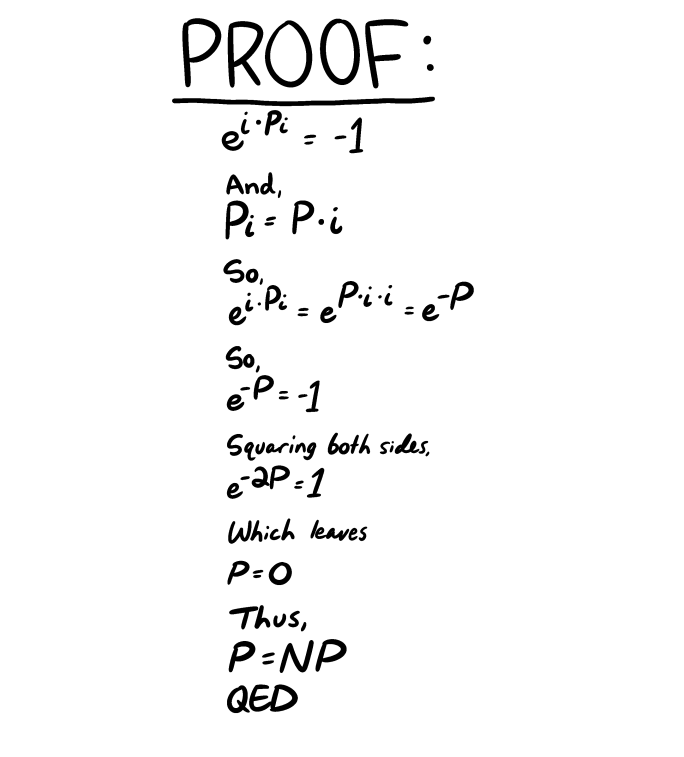
\includegraphics[scale=0.2]{smbc_comic}\footnote{\url{http://www.smbc-comics.com/?id=3919}}
\end{center}
\end{frame}

\begin{frame}
\begin{center}
\frametitle{The end}
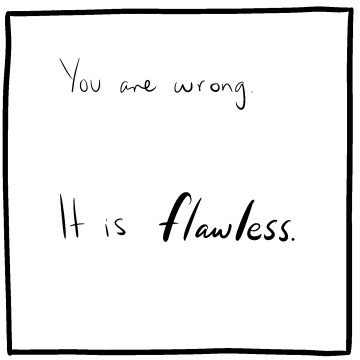
\includegraphics[scale=0.5]{smbc_comic_votey}\footnote{\url{http://www.smbc-comics.com/?id=3919}}
\end{center}
\end{frame}

%----------------------------------------------------------------------------------------

\end{document} 
